%%%%%%%%%%%%%%%%%%%%%%%%%%%%%%%%%%%%%%%%%%%%%%%%%%%%%%%%%%%%%%%%%%%%%%%%
\section{Introduction}\label{sec:intro}
%%%%%%%%%%%%%%%%%%%%%%%%%%%%%%%%%%%%%%%%%%%%%%%%%%%%%%%%%%%%%%%%%%%%%%%%

\subsection{The problem}

A \emph{meander of order $n$} is a closed road that crosses a straight river $2n$ times and
never crosses itself. Two drawings are the same meander if one can be deformed into the other
without changing the order of the crossings along the river. The number of meanders of order
$n$ is $M_n$:
\[ M_1, M_2, \ldots \;=\; 1,\ 2,\ 8,\ 42,\ 262,\ 1828,\ 13820,\ 110954,\ \ldots \]
Figure~\ref{fig:meander} shows one of the eight meanders of order $3$. Exact values have been
computed for every $n\le 32$~\cite{JG,JensenGit}; values for $33\le n\le 40$ have also been
computed privately, but they are not published or independently checked. No formula for $M_n$
is known.

\begin{figure}[t]
\centering
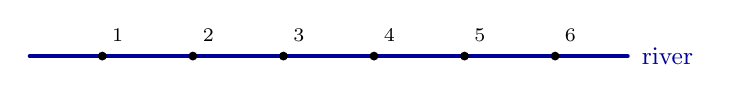
\begin{tikzpicture}[x=1.15cm,y=0.62cm,line cap=round]
  \draw[blue!60!black,line width=1.6pt] (0.2,0)--(6.8,0);
  \node[blue!60!black,anchor=west] at (6.85,0) {\small river};
  \begin{scope}[line width=1.1pt]\meanderroad\end{scope}
  \foreach \k in {1,...,6} {\fill (\k,0) circle[radius=1.6pt]; \node[fill=white,inner sep=0.6pt,font=\scriptsize] at (\k+0.17,0.42) {\k};}
\end{tikzpicture}
\caption{A meander of order $3$. Above the river the road joins crossings $1$--$2$, $3$--$6$
and $4$--$5$; below it joins $1$--$6$, $2$--$5$ and $3$--$4$. Following the road from
crossing $1$ visits $1,2,5,4,3,6$ and returns to $1$.}
\label{fig:meander}
\end{figure}

The numbers are believed to follow the law
\begin{equation}\label{eq:law}
M_n \;\approx\; A\,\mu^n\, n^{-\alpha}
\end{equation}
for constants $A$, $\mu$ and $\alpha$, in the sense that the ratio of the two sides should tend to
one as $n\to\infty$. The two main constants carry different information.

\begin{itemize}
\item The growth rate $\mu=\lim M_n^{1/n}$ exists. Intuitively, a meander offers about $\mu$
choices each time its order grows by one, that is, for each further pair of crossings.
Extrapolation from the exact counts gives $\mu\approx 12.2629$, and the best proved bounds are
$12.2191\le\mu\le12.2970$ (Paper~B; see Section~\ref{sec:tape}).
\item The exponent $\alpha$ is a slow correction on top of the exponential growth. It measures
how much of the naive count $\mu^n$ survives the global requirement that the road closes into a
single loop. Physicists predict~\cite{DGG} that $\alpha$ equals
\begin{equation}\label{eq:alpha}
\alpha_* \;=\; \frac{29+\sqrt{145}}{12} \;\approx\; 3.4201,
\end{equation}
and numerical fits to the exact counts are consistent with it to about three decimal places
(Section~\ref{sec:estimate}). This is not proved. Throughout,
$\alpha$ denotes the true exponent, whatever it is, and $\alpha_*$ the predicted number.
\end{itemize}

The growth rate depends on every detail of the definition, while the exponent is expected to be
\emph{universal}: it should not change if the rules are altered in small ways
(Section~\ref{sec:walks}). The predicted value is also irrational, which has a concrete
consequence. For the exponentially bounded integer coefficients considered here, a linear differential equation
with polynomial coefficients would impose rational local exponents through the theory of
$G$-functions~\cite{Andre}. In the power-law setting above, this forces $\alpha$ to be rational;
Paper~C gives the precise argument. So if $\alpha=\alpha_*$, the generating function
$\sum M_n x^n$, the power series whose coefficients are the counts, satisfies no such equation,
and the usual exact methods of enumeration cannot reach it.

\subsection{What is known, and the papers of this series}

Write $u_n=M_n/\mu^n$ for the factor left over once the exponential growth is removed. The
prediction says $u_n\approx A\,n^{-3.4201}$. Table~\ref{tab:window} lines up what is proved.

\begin{table}[h]
\centering
\begin{tabular}{lll}
\toprule
 & lower bound & upper bound \\
\midrule
growth rate $\mu$ & $12.2191$ (Paper~B) & $12.2970$ (Paper~B) \\
proved for meanders: $u_n$ & $u_n\ge e^{-C\sqrt n}$ (Paper~C) & $u_n\le \mu/(8n)$ (Paper~C) \\
predicted: $u_n$ & $u_n\approx A\,n^{-3.4201}$ & $u_n\approx A\,n^{-3.4201}$\\
near-splits in the limit & exponent $3.4201$ (Paper~D) & exponent $3.134$ (Paper~D)\\
\bottomrule
\end{tabular}
\caption{What is proved, and what is predicted. The first row bounds the growth rate; the best
numerical estimate is $12.2629$. The middle rows concern the leftover factor $u_n=M_n/\mu^n$; $C$
is a constant. The last row concerns
the probability of a near-split in the conjectured limit of large meanders: an approximate
version of a meander splitting into two halves at the middle of the river
(Section~\ref{sec:limit}). Its predicted exponent is $\alpha_*$, and an exponent closer to
$\alpha_*$ is better on either side.}
\label{tab:window}
\end{table}

This paper is the first of four. It explains the intuition and surveys the results; the other
three contain the new results with their proofs. Here and below, a factor $n^{o(1)}$ is one that
grows more slowly than every positive power of $n$ and decays more slowly than every negative
power.
\begin{itemize}
\item \textbf{Paper~B}~\cite{PaperB}: \emph{the tape machine and bounds on the growth rate.} A
meander is encoded exactly by a walk on words in two letters that returns to its start
(Section~\ref{sec:tape}). Positive weights on these words give the upper bound, and a random rule
for choosing the steps of the walk gives the lower bound; together,
$12.2191\le\mu\le12.2970$, certified by exact computer checks.
\item \textbf{Paper~C}~\cite{PaperC}: \emph{the subexponential factor.} For meanders themselves,
as opposed to continuum models, $\mu^n e^{-C\sqrt n}\le M_n\le \mu^{n+1}/(8n)$
(Section~\ref{sec:proved}). Both bounds are new as far as we know; the lower bound improves one
obtained earlier in this project, which had an extra factor $\log n$ in the exponent. Paper~C also
contains an exactly solvable family of meanders with an irrational exponent
(Section~\ref{sec:band}), and precise statements of what would improve the bounds.
\item \textbf{Paper~D}~\cite{PaperD}: \emph{continuum results.} Ang, Park, Pfeffer and Sheffield
introduced a continuum model of random surfaces in which a surface is built from small squares
and its size is the number of squares. The continuum analog of the number of spanning trees (sets
of edges that reach every vertex without forming a loop) is a determinant. They proved that, among
surfaces with a given number of squares, weighting each surface by a power of this determinant
changes the model's single parameter by an exact amount. Paper~D supplies the normalization that
compares surfaces of different sizes, and proves how the probability that the surface has at least
$n$ squares decays with $n$. Together these show that, in this model, when surfaces are weighted
by the analog of two spanning trees, the total weight of surfaces with at least $n$ squares decays
like $n^{-x_2+o(1)}$, with $x_2=(17+\sqrt{145})/12$. This tail exponent corresponds to the
counting exponent $1+x_2=\alpha_*$ (Section~\ref{sec:continuum}).

Paper~D also studies the random surface that Borga, Gwynne and Sun conjecture to describe large
meanders (Section~\ref{sec:limit}). A meander of order $2m$ has a \emph{thin neck at the middle}
if the road crosses a vertical line through the middle of the river only twice; cutting along
the line then splits it into two meanders of order $m$. A \emph{near-split} is the continuum
version of such a neck, allowed to be imperfect by a fraction $\delta$ of the surface. Paper~D
proves that its probability is at least a constant times $\delta^{\alpha_*}$, the predicted
order, and at most a constant times $\delta^{3.134}$. Finally, Paper~D shows what a comparison
between finite meanders and the limit would give, for example
$M_n\ge\mu^n n^{-\alpha_*-o(1)}$ (Section~\ref{sec:bridge}).
\end{itemize}
Earlier exact formulas for related families are collected in~\cite{ExactPaper}.

\subsection{How the paper is organized}

The first half explains where~\eqref{eq:alpha} comes from. Section~\ref{sec:walks} shows the same
kind of exponent for random walks, where everything can be computed, and explains universality.
It then describes two ways to read a meander as a walk. Section~\ref{sec:surfaces} turns a
meander into a random surface with two curves drawn on it and explains the formula that produces
$3.4201$.

The second half surveys what is proved. Section~\ref{sec:proved} treats finite meanders.
Section~\ref{sec:continuum} describes the continuum model in which the KPZ formula, the rule
behind~\eqref{eq:alpha}, is a theorem.
Section~\ref{sec:limit} describes the conjectured limit of large meanders.
Section~\ref{sec:bridge} explains the missing step, from the continuum back to finite meanders,
by comparison with percolation (a classical model of random clusters on a lattice, where the
same step was carried out), and lists open problems.

\subsection{Status of the results}

The background in Sections~\ref{sec:walks} and~\ref{sec:surfaces} is either classical or a
physical prediction, and we say which. Except where noted, every result of the project quoted here
is new as far as we know, and each is proved in Paper~B, C or D, with a pointer to the complete proof in the project repository~\cite{Repo},
except one result on meandric systems in Section~\ref{sec:shape}, whose proof is only in the
repository. Most of these proofs were checked by at least one separate, independent reading; each
paper says which were not, and we repeat this where it matters. Nothing has been reviewed
outside the project. This paper gives short arguments where they explain something and
otherwise points to the paper that has the proof. Appendix~\ref{app:repo} says where in the
repository the proofs and data are.
